\documentclass[11pt]{article}

\usepackage{
	setspace,
	fullpage,
	multicol,
	float,
	amsmath,
	graphicx} 
%\doublespacing

\floatplacement{figure}{H}

% Citation style in the text: numbers in parenthesis, sorted by their
% order in the list of references. Uses ranges: (1-3), not (1,2,3)
\usepackage[round,numbers,sort&compress]{natbib} 

% Bib style requires biophysj.bst be in the document directory
\bibliographystyle{biophysj}
% Numbering style in the list of references: number followed by period
\renewcommand{\bibnumfmt}[1]{#1.}

\title{Crossbridges are hard, or rather, stiff}
\author{
	C.~Dave,$^{\dagger \ast}$~
	Mikey,$^\ddagger$~
	and TommyD$^\S$\\ 
	\small 
	$^\dagger$Department of Physiology and Biophysics, University of Washington, and 
	$^\ddagger$Department of Bioengineering, University of Washington, and 
	$^\S$Department of Biology, University of Washington, Seattle, Washington \\
	$^\ast$Correspondence: cdave@u.washington.edu
	\normalsize
}

% Revision date - uncomment to exclude date in the final version
\date{}
% Running head
%\pagestyle{myheadings}
%\markright{XBs are Hard}

\begin{document}

%\maketitle
{\fontfamily{phv}\selectfont

\LARGE
\noindent \textbf{Multidimensional Crossbridges: Not a rope of sand }\\

	\large
	\noindent C.~Dave,$^{\dagger \ast}$~
	Mikey,$^\ddagger$~
	and TommyD$^\S$\\ 
	\small 
	$^\dagger$Department of Physiology and Biophysics, University of Washington, and 
	$^\ddagger$Department of Bioengineering, University of Washington, and 
	$^\S$Department of Biology, University of Washington, Seattle, Washington \\
	$^\ast$Correspondence: cdave@u.washington.edu \\
	\normalsize


\noindent \emph{Abstract:} 
Lorem ipsum dolor sit amet, consectetur adipiscing elit. Fusce id quam et odio viverra fermentum. Donec tincidunt faucibus justo id ultricies. Pellentesque quis quam risus, nec sollicitudin nibh.   \\[.5em]
{\footnotesize \emph{
Keywords: myosin; spatially-explicit model; crossbridge kinetics}} \\[.5em]
 {\footnotesize \textbf{
 Author Summary: Models of muscle contraction have long treated the molecular motor myosin as a simple spring oriented parallel to its direction of movement. This does not allow for the investigation of phenomena such as the perpendicular force observed during shortening, or the dependence of the maximum force produced on spacing between the contractile filaments that comprise muscle. We demonstrate an alternative model, computationally simple enough to use in large networked models, that incorporate both linear and torsional or angular springs. These models capture much of the behavior missing from pervious efforts.}}} \\


\begin{multicols}{2}



\section*{Introduction}

Sarcomere-scale modeling of muscle contraction has largely changed since the introduction of the sliding crossbridge model in the 1950s, but the geometry of the individual crossbridges used has remained largely unaltered. While thermodynamic account had been introduced to the crossbridge kinetics, compliance has been introduced to the filaments, and multiple filaments have been arranged to mimic the lattice, the one dimensional single spring nature of the crossbridge has continued to be used as a model of the mechanism of force generation.

\paragraph*{History of Models}

\paragraph*{Increasing knowledge of myosin}

\begin{figure}[H]
\begin{center}
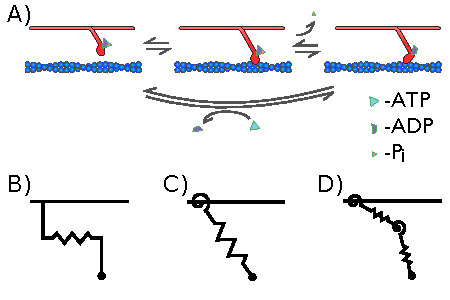
\includegraphics{../imgs/XBCycle.pdf}
\label{xbtypes}
\caption{{\small Kinetic scheme and crossbridge types under investigation. A) Three state kinetics used in most models and extended here. B) Single spring crossbridge model used in models since \cite{Huxley57}. C) Two spring system, consisting of a torsional/angular spring and a linear spring. D) Four spring system using two torsional and two linear springs.}}
\end{center}
\end{figure}


\section*{Materials and Methods}



\subsection*{Historical 1-D Crossbridge}
\paragraph*{Geometry and Force/Displacement Equations}

\begin{equation}
U(r)=\frac{1}{2}k_r (r-r_0)^2
\end{equation}

\begin{eqnarray}  
	r_{12}(r, \theta) & = & 0.001 + 0.5 * (1 + \tanh( \nonumber \\
				&   & 0.6 (U_1(r, \theta) - U_2(r, \theta)))) \\
	r_{20}(r, \theta) & = & e^{-1 / U_2(r, \theta)}
\end{eqnarray} 
 
\paragraph*{Kinetics: Equations and Figures}

\subsection*{A 2-D 2-Spring Crossbridge}

\paragraph*{Geometry and Force/Displacement Equations}

\begin{equation}
U(r,\theta)=\frac{1}{2}k_r (r-r_0)^2+\frac{1}{2}k_\theta (\theta-\theta_0)^2
\end{equation}

\paragraph*{Kinetics: Equations and Figures}

\paragraph*{Cutting out cross-sections}

\subsection*{A 2-D 4-Spring Crossbridge}
\paragraph*{Geometry and Force/Displacement Equations}
\begin{eqnarray}
	\lefteqn{U(\phi,\ell,r,\theta) = }  \nonumber \\
 	& & \frac{1}{2}k_\phi (\phi-\phi_0)^2 + \frac{1}{2}k_\ell (\ell-\ell_0)^2 + \nonumber \\
	& & \frac{1}{2}k_r (r-r_0)^2 + \frac{1}{2}k_\theta (\theta-\theta_0)^2
\end{eqnarray}

\paragraph*{Kinetics: Equations and Figures}
\paragraph*{Cutting out cross-sections}


\section*{Results}


\section*{Discussion}

\subsection*{Lattice Spacing Dependence of Binding Rates}


\subsection*{Forward Biased Binding}


% Compile and format the bibliography (bj_bibtex_template.bib BibTeX
% file must be present in the document directory)
%\bibliography{bj_bibtex_template}

% closing statement, nothing below matters
\end{multicols}
\end{document}
